\documentclass[11pt,english]{article}
\usepackage{ae,aecompl}
\usepackage{helvet}
\usepackage[T1]{fontenc}
\usepackage[authoryear]{natbib}
\usepackage{multirow}
\usepackage{amssymb,amsmath,amsthm}
\usepackage[nolists]{endfloat}
\usepackage{graphicx}
\usepackage[pdfborder={0 0 0}]{hyperref}
\usepackage{chngpage}
\usepackage{pdflscape}
\usepackage{pdfpages}
\usepackage{fullpage}
\usepackage{setspace}
\usepackage{booktabs}
\usepackage{subfigure}
\usepackage{colortbl}
\usepackage[small,compact]{titlesec}
\usepackage{rotate}

\doublespacing

\newcommand{\noun}[1]{\textsc{#1}}
\newcommand{\citetapos}[1]{\citeauthor{#1}'s \citeyearpar{#1}}
\providecommand{\tabularnewline}{\\}

\theoremstyle{plain} \newtheorem{claim}{Claim}
\theoremstyle{plain} \newtheorem{prop}{Proposition}
\theoremstyle{plain} \newtheorem{hypo}{Hypothesis}

\bibpunct[: ]{(}{)}{;}{a}{,}{,}

\begin{document}

\title{Renewable energy and sustainable development: a case study on impact of climate change on hydropower in Vietnam \thanks{We thank Professor Wolfram Schlenker for research guidance. The research was sponsored by the Global Green Growth Institute.}}

\author{Anthony D'Agostino\\Columbia University \and Ruinan Liu\\Columbia University \and James Rising\\Columbia University \and Semee Yoon\footnote{Corresponding author. Address: 420 West 118th Street, 712 International Affairs Building. New York, NY 10027, USA. Tel: +1-646-592-0813. Email:sy2229@columbia.edu.}\\Columbia University }

\maketitle

\begin{center}
\textbf{Incomplete and preliminary. \\
Please do not cite. }
\end{center}

%\begin{abstract}

%\end{abstract}

\textbf{Keywords}: hydropower, dams, renewable energy, energy access, climate change, Vietnam

\clearpage

\section{Introduction}

	Since the introduction of Doi Moi (renovation) reforms in the 1980s, Vietnam has experienced economic growth as the government encouraged the transition from a centralized economy to a decentralized economy with an active private sector. GDP per capita increased from \char36 98 in 1990 to \char36 1596 in 2012 (both in 2012 USD). Industrial value added as the percent of GDP increased from 23\% in 1990 to 40\% in 2012. The growth rate of GDP from 1990 to 2012 is about 21\%. The percent of population living in urban areas has moderately increased from 24\% in 1990 to 32\% in 2012 \citep{WorldBank2014}. Given the projections on future economic growth, Vietnam needs to secure adequate electricity provision to meet demand from both industrial and household sectors. 

	Electricity consumption in Vietnam has almost quadrupled from 22,000 GWh in 2000 to 86,000 GWh in 2010. As of August 2013, the cost of electricity is 7.1 cents/kWh (one of the more affordable/expensive in the region). Vietnam currently relies on hydropower, coal and natural gas as sources of electricity generation. The heavy reliance on hydroelectric power, which constitutes 40\% of electric capacity and 25\% of electricity output, is an urgent issue that should be addressed in detail, considering the environmental and social consequences of unsustainable management. 

	With this complexity in mind, we will focus on the evolution of dam infrastructure along the Mekong River, which is driven by many forces, including climate change, economic development, and cross-boundary water availability and politics. To provide a blueprint for Vietnam's hydropower sector, we need to try to understand how these forces will each develop over both time and space. To research the social and political dynamics behind dam projects, we will use spatial future demand for hydropower electricity and irrigation. While there is some research on future hydrological projections for the Mekong due to climate change, there has not been an attempt to look at conseequences of hydrological variability in consideration of demand for electricity and climate change predictions in the Mekong. Thus, results from this research may have important implications for agricultural and industrial activities in Vietnam, which is located in the lower Mekong River. 
	
	For thorough understanding of the status quo, we will analyze the current water availability and flow in Southeast Asia (Vietnam, Cambodia, Laos and China) for information on the environmental aspect of the situation at hand. This analysis will be useful to look at the interplay between changes in meltwater for hydropower and further upstream hydropower in adjacent countries. Then, using dynamic modeling results for volatility for 2050 and 2100, we will look into the relationship between water resource management and electricity generation. 

	Given these results from the first stage of the project period, we will also look at political and societal linkages between dams for hydropower and irrigation to find room for co-management. For this next step of focus group meetings, we will run a workshop with policy makers and water experts in Vietnam and see how they respond to the results to see changes in decision-making. 
	
	The remainder of this section discusses the literature on drivers of dam management in policy-making. Section 2 provides the detailed research plan. Section 3 provides data used for hydrological information in the Lower Mekong Delta. Section 4 provides hydrological information of the lower Mekong. Section 5 addresses next steps. 

\subsection{Literature Review}

Research on water management in the Mekong can be generally categorized to two ideas: (1) scientific analysis of environmental impact on the Mekong River Basin due to climate change or hydropower development and (2) qualitative analysis on politics of the Mekong region. 

% AD: to what degree do we want to get involved in this politics literature?  

% group 1 papers \citep{Rasanenetal2012; Laurietal2012; Zivetal2012}
% group 2 papers \citep{Lebeletal2005; }

Several studies have used output from General Circulation Models (GCMs) to forecast hydrological impacts of climate change for the Mekong region. \citet{Vastila:2010bz} input precipitation data from the PRECIS regional climate model into hydrological, ocean circulation, and floodplain models to estimate discharge flows at Kratie for 2010-2049, finding annual discharge rates higher than historical data, but with smaller variance.  \citet{Lauri2012HESSD} find that in next two, three decades the change in discharge at Kratie, Cambodia will be between - 11\% to +15\% during the wet season and  - 10\% to +13\% during the dry season. Moreover, changes in discharges are expected to have a varying impact on reservoir operations. Changes in dry season flows are expected to range between 25 - 160\% and changes in flood peaks are expected to be 5 - 24\% lower. (WHICH?) Authors note that such changes in reservoirs will have an influence on aquatic ecosystems.     THE SOCIAL IMPACTS OF THESE CHANGES ARE EXPECTED TO BE ...   need to include EASTHAM et al. 2008   Nuorteva et al. 2010 

Ecologists use ecological models to study the impact of dams on the Mekong River Basin, which is the largest inland fishery in the world that provides home to about 65 million people.  Using information on fish resources, power production,  and trade-off between dam locations, \citet{ZivPNAS2012} find that completion of 78 dams on the tributaries of the Mekong River Basin will have highly detrimental impact on fish productivity and biodiversity of the aquatic ecosystem. 

Analysis of water resources governance and policy-making of the Mekong region is complex in the diversity of actors at play across scales and levels. At the national level, six governments are involved: Vietnam, Cambodia, Lao PDR, China's Yunnan Province, Myanmar and Thailand. Since decisions made at the national level have direct impact on household livelihoods, decision-making in the political arena need to consider multi-level interests. \citet{Lebel2005} address complexity using issues of scale regarding place and position. \citet{Kuenzer2012SS} focus on the discrepancies between upstream and downstream countries in the impacts of hydropower development. 

HYDROPOWER IN THE ERA OF CC 
Furthermore, climate change presents a range of challenges to existing dam infrastructure, including threats of dam failure caused by magnified flood risks \citep{Pittock:2011fv}.  IMPACTS ON MARINE LIFE.    

LIT ON HYDRO-PLANNING MORE BROADLY? 

\section{Research Plan}

This research is carried out in two phases. 

In phase 1, we will acquire dam and historical flow data from throughout the Mekong basin. We will also collaborate with a hydrological team to apply an appropriate physical or statistical model to predict flows using historical and CMIP5 precipitation data, in the presence of the dams.  We will also have time-series data on electricity demand in China to help estimate the flow management of the dams. Then, we will provide a model of spatiotemporal model hydropower electricity and dam irrigation demand throughout the Mekong, accounting for electricity and irrigation supply from other sources.  Treating each country as an independent regulatory body, we would identify the stochastic sequence of dam infrastructure projects that each country might engage in, whereby downstream countries must respond to upstream flow changes.

In phase 2, we will present our results from phase 1 to decision-makers on dam construction and water supply systems of Vietnam during focus groups to see if scientific information plays a role in policy decisions. Often times, decisions on infrastructure investment are made without consideration of vulnerability of future energy use, projected population growth, and urban/rural composition.  

\subsection{Research schedule}
The study is implemented as follows:
\begin{enumerate}
	\item Baseline research of streamflow and hydropower generation of Vietnam in March, April, and May 2014.
	\item Baseline analysis of electricity demand in Mekong region in April and May 2014.
	\item Dam location modeling in May - June 2014.
	\item Prepare focus group questionnaires in May 2014.
	\item Visit Can Tho University (near Hanoi) in July 12-14, 2014.
	\item Visit government officials in Ho Chi Minh from July 15 to 19, 2014.
	\item Finish write-up of the impact of scientific information on policy making from mid-July to August 2014. 

\end{enumerate}

\section{Data Sources}

Due to great interest on both national and international level regarding economic and environmental potential of the Mekong region, data on hydrology and dam project development is available through multiple sources. 

Streamflow data used in the first stage is from the digital database of the Mekong River Commission. Data from Tan Chau station in Vietnam covers 1969 to 2006. 

Another source of streamflow data is the data library of the International Research Institute for Climate and Society within the Earth Institute of Columbia University. There is both yearly and monthly streamflow data from 1920 to 1987. 

\section{Hydrology}

Figure \ref{discharge} shows the annual mean discharge in the Mekong Basin between 1920 and 1990 using IRI data. Gauges that are on smaller streams (red and black) show greater variability and those on the main river (blue and green).

\begin{figure}
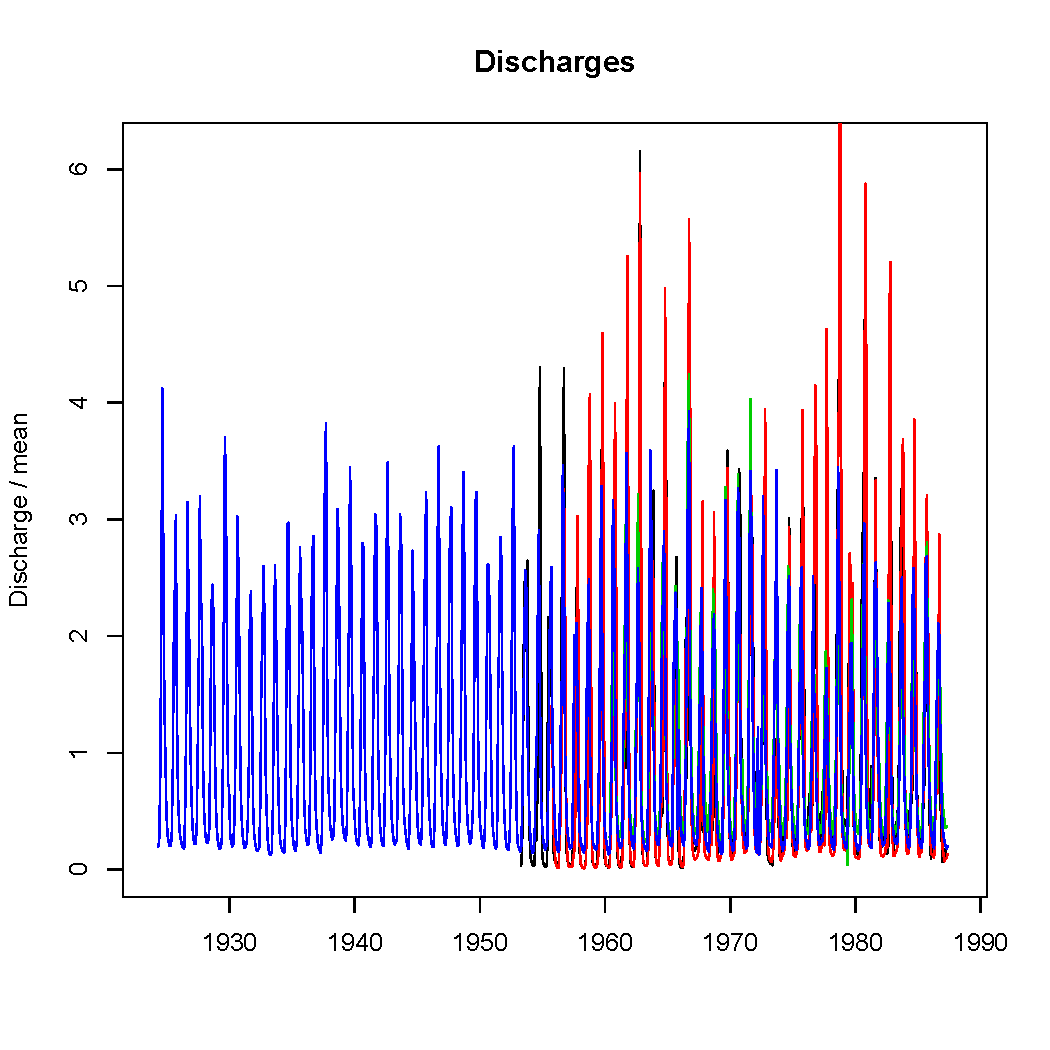
\includegraphics{displays/discharge_time.pdf}
\label{discharge}
\caption{Monthly Discharge Rates for four gauges in the Mekong Basin (m$^3 s^{-1})$} 
\end{figure}
 
Figure \ref{bottom} shows discharge statistics for the lowest of these four gauges, Ubon Ratchathani, in $m^3 s^{-1}$. % 890
All three curves-- the yearly minimum, mean, and maximum flow-- show slight upward trends in time, suggesting an increase in precipitation over the region.
 
\begin{figure}
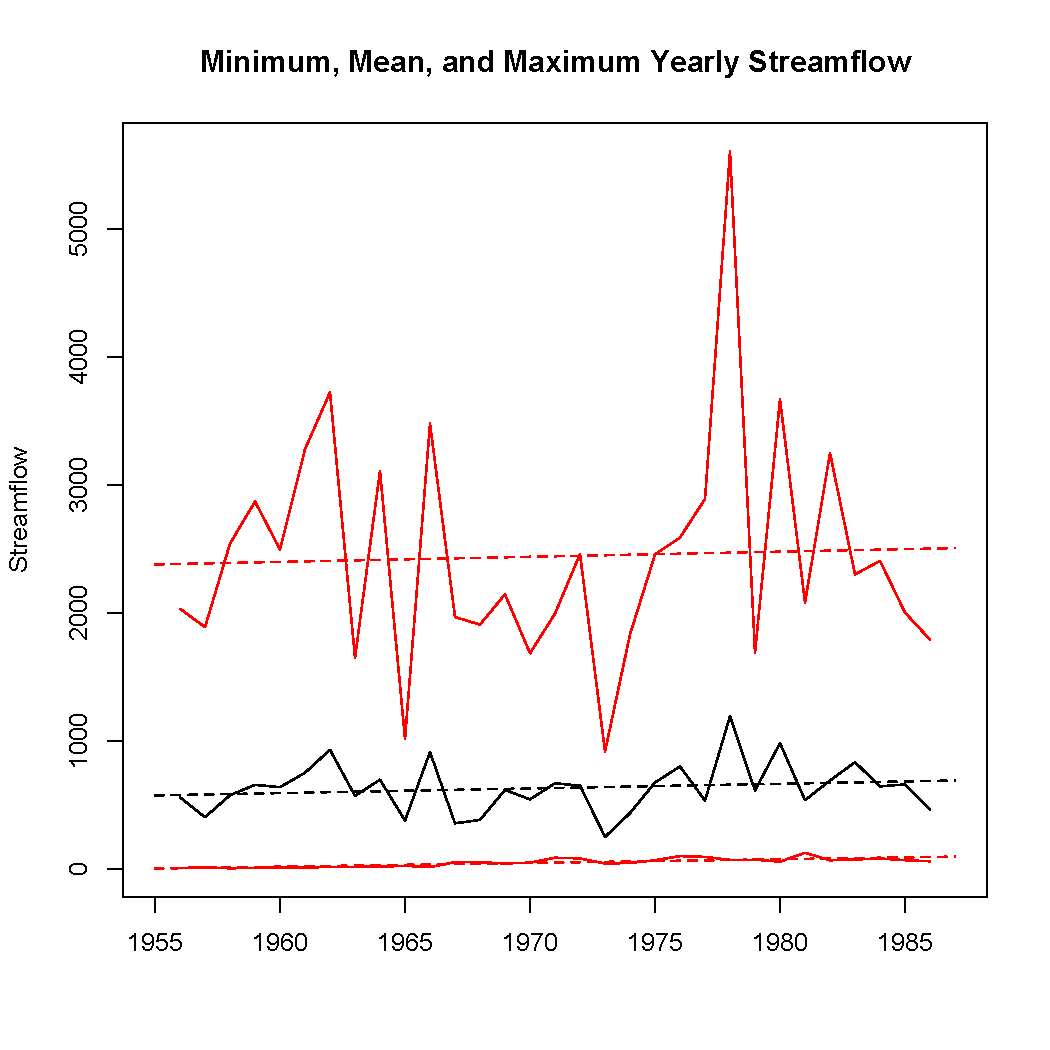
\includegraphics{displays/bottom-year.pdf}
\label{bottom}
\caption{Minimum, Mean, and Maximum Yearly Streamflow for Ubon Ratchathani, Thailand, near the Mekong delta $(m^3 s^{-1})$.  Flows have shown a slow increase over time, perhaps due to climate change.}
\end{figure}

Figure \ref{diff} shows difference in the dischage between two gauges along the Mekong.  % 1248 - 891
The maximum discharge difference decreases over time.  This is the opposite that one would expect from flood management, where downstream flows should be more buffered from upstream variation.

\begin{figure}
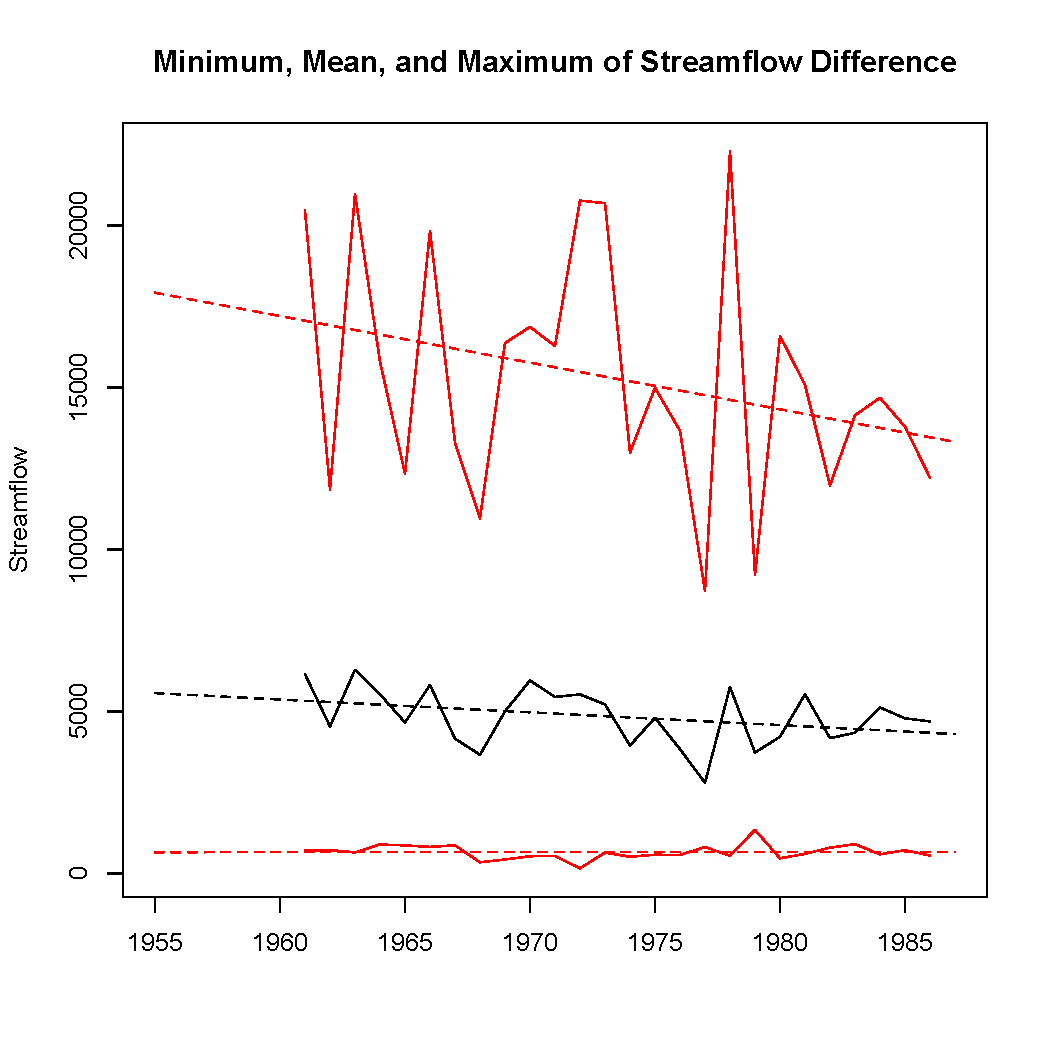
\includegraphics{displays/difference-year.pdf}
\label{diff}
\caption{Minimum, Mean, and Maximum Yearly Streamflow Difference between Mukdahan Thailand and Chiang Saen, Thailand $(m^3 s^{-1})$.  Extreme differences have been decreasing over time.}
\end{figure}

\section{Electricity Generation}

Given the importance of hydropower for Vietnam's power generation, we expect streamflow to be a weak predictor of power generation.  The right graph in figure \ref{fig:loggen} shows the smooth, linear rise of logged power generation in Vietnam.  The left graph seeks to explain the detrended energy generation using maximum yearly streamflow for the Tan Chau gauge station, near the border between Vietnam and Cambodia on the lower Mekong.

\begin{figure}
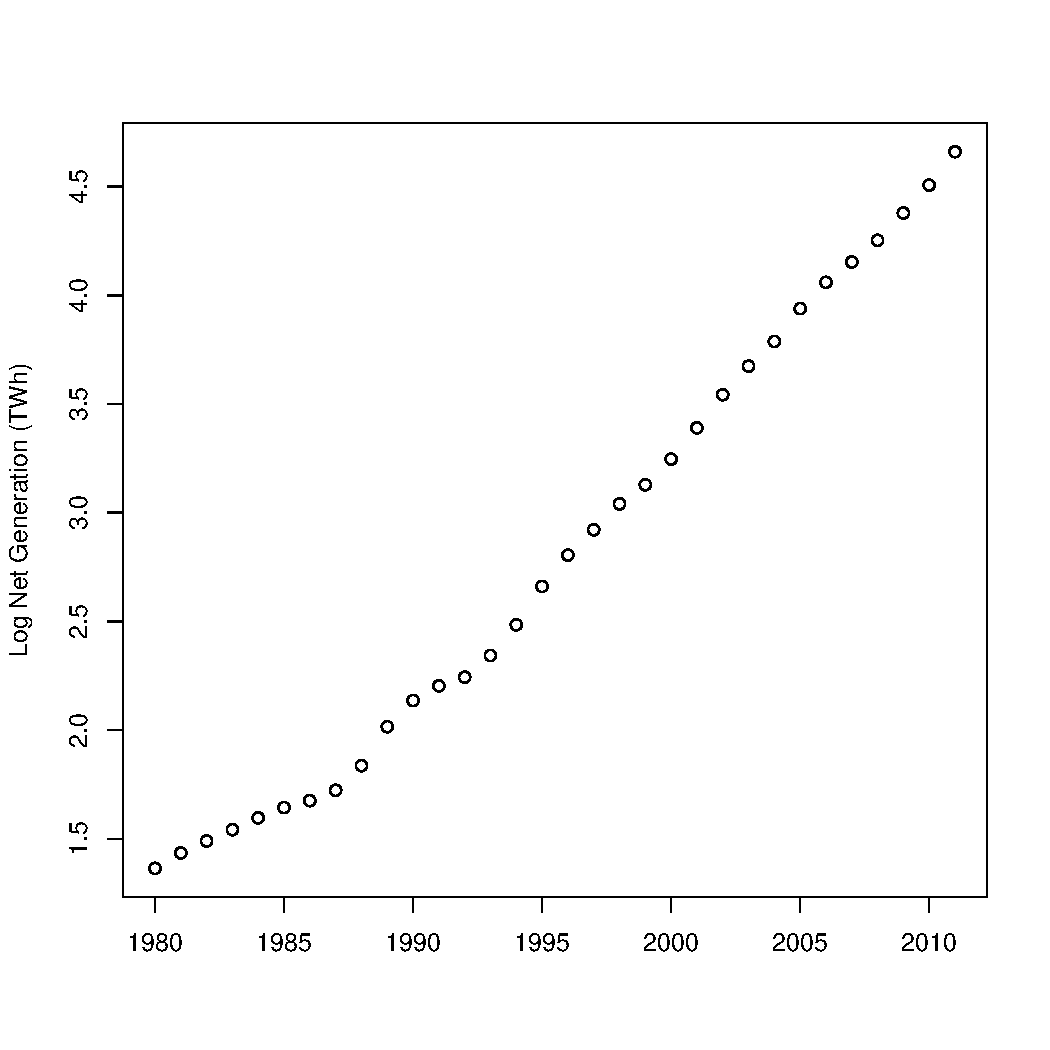
\includegraphics[width=3in]{displays/loggen.pdf}
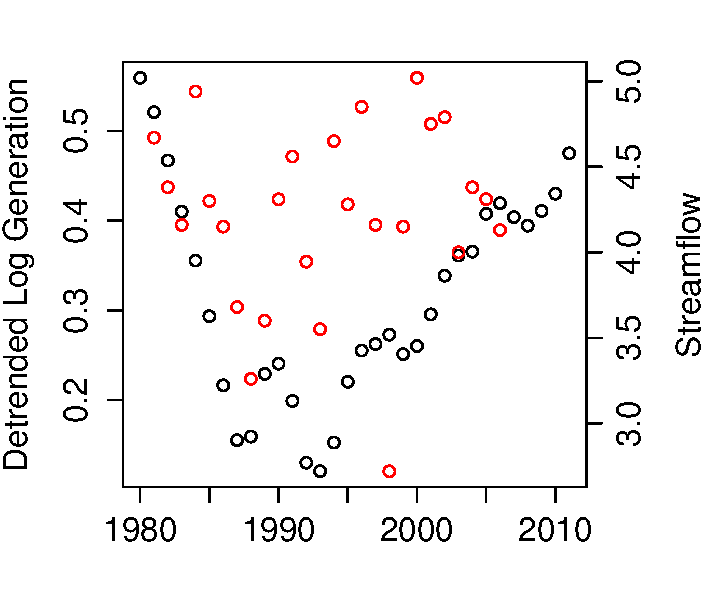
\includegraphics[width=3.4in]{displays/correlation.pdf}
\label{fig:loggen}
\caption{Electricity Production and Streamflow.  {\bf Left:} Log power generation has increased nearly linearly since 1980, so the deviations from this trend might be explained by varying hydropower potential. {\bf Right:} Streamflow and deviations from the linear trend in log-space have a statistically-significant, but low, correlation.}
\end{figure}

\section{Next steps}

In the second phase of the research, we will conduct a focus group to ask and encourage discussion about factors considered for hydropower management and policy-making. The survey composes of three parts: decision-making process, climate change, and interviewer information. 

\subsection{Focus group survey}

\textbf{Part 1. Decision making process}

\begin{itemize}
\item[] 101 In what capacity did you take part in the decision making process? 

\item[] 102 Where do you get information about criteria to decide on dam construction? 
 
\item[] 103 Who do you think are important institutional bodies that decide on dam construction? 

\item[] 104 Have you made a decision to build dams in the last year? 

\item[] 105 Have you made a decision to build dams in the last five years?

\item[] 106 How long does a typical dam project planning take? 

\item[] 107 Are dams put in place proactively or retroactively (in response to increased demand for energy)?

\item[] 108 What are the biggest planning obstacles to completion of a successful dam project? [e.g. because of relocation, optimal sites cannot be selected? ]

\item[] 109 How do you balance irrigation and/or hydropower generation? 
[What guides multiple objective decision making?  ]

\item[] 110 How is the master plan for the Mekong basin devised for a 5-year or decade year ?

\item[] 111 How do you perceive cross-boundary issue of hydro management? 

\item[] 112 What are some long-term issues that you think hydrological policy needs to address beyond economics? 

\item[] 113 What are the principal stressors related to integrated resource management affecting the Mekong Delta? [note: Economic, policy, environmental, and social/cultural stressors should be considered. These stressors should be considered on various scales ranging from local to global.]

\end{itemize}

\textbf{Part 2. Climate change}

\begin{itemize}
\item[] 201 How concerned are you about climate change?

 \renewcommand{\labelenumii}{\Roman{enumii}}
\begin{enumerate}
  \setcounter{enumii}{4}
\item Not interested at all
\item Slightly interested
\item Moderately interested
\item Very interested
\end{enumerate}

\item[] 202 Can you situate climate change with other aspects of society, relative to dam management faces? 

\item[] 203 How is climate change related to the work you deal with in the agency? 

\item[] 204 Has climate change impacted your day-to-day life? 

\item[] 205 Do they use information about climate change in long-term planning? 

\item[] 206 Do you communicate with other agencies about dam sites and strategies for hydropower management? 

\end{itemize}

\textbf{Part 3. About the interviewee}

\begin{itemize}
\item[] 301 How much of your agency/department's programs is related to hydropower production? 

\item[] 302 What are the long-term goals for electrification at your agency? 

\item[] 303 What are the long-term goals for green energy at your agency? 

\item[] 304 What is your age?

\item[] 305 Do you have any children? 

\item[] 306 What is the highest level of education you have obtained? 

\item[] 307 How many people live in your household? 

\item[] 308 Annual household income (provide ranges to choose from )

\item[] 309 When you have heard about proposed projects where there is a conflict between development and the environment, have you tended to:
\begin{enumerate}
\item favor protection of the environment
\item favor development and environment protection about equally
\item favor development
\end{enumerate}
\end{itemize}

\subsection{Who to meet}

The list of potential people to meet includes: 
\begin{itemize}
\item	Representative of the Ministry of Construction, which has the primary technical oversight of the water sector in urban areas. 
\item	Representative of the Ministry of Agriculture and Rural Development, which has the primary responsibility over the water sector in rural areas. 
\item	Representative of the Ministry of Natural Resource and Environment (MNRE) and/or its provincial departments. They are in charge of management and monitoring the quality and quantity of surface water and ground water resources. MNRE also collects environmental fees on polluted water. 
\item	Representative of the Ministry of Planning and Investment and the Ministry of Finance, which decide on the financial factors in water sector development. 
\item	People's Committees at the province level, which defines and delegates water management roles to departments within the appropriate administrative level for implementation (same for district and commune). 
\item	Department of Planning and Investment helps to direct investments in water sector in cooperation with other departments.
\item	Department of Construction helps to manage water supply at the corresponding localities. 
\end{itemize}


\clearpage

\bibliographystyle{../apsr2}
\bibliography{../dams,../ald_ref}

\end{document}
